\documentclass[fleqn,10pt]{wlscirep}
\usepackage[utf8]{inputenc}
\usepackage[T1]{fontenc}
\usepackage{amsmath,amssymb}
\usepackage{booktabs}
\usepackage{multirow}
\usepackage{graphicx}
\usepackage{subcaption}

\title{HSANet: Uncertainty-aware brain tumor classification using hybrid scale-attention networks with evidential deep learning}

\author[1,*]{Md. Assaduzzaman}
\author[1]{Md. Tareque Jamil Josh}
\author[1]{Md. Aminur Rahman Joy}
\author[1]{Md. Nafish Imtiaz Imti}

\affil[1]{Department of Computer Science and Engineering, Daffodil International University, Daffodil Smart City, Ashulia, Dhaka 1341, Bangladesh}

\affil[*]{assaduzzaman.cse@diu.edu.bd}

\begin{abstract}
Accurate classification of brain tumors from magnetic resonance imaging (MRI) is essential for treatment planning in neuro-oncology, yet existing deep learning methods lack principled uncertainty quantification critical for clinical decision support. Here we present HSANet, a hybrid scale-attention network integrating adaptive multi-scale feature extraction, dual attention mechanisms, and evidential deep learning for uncertainty-aware classification. The Adaptive Multi-Scale Module employs parallel dilated convolutions with learned fusion weights enabling dynamic receptive field adjustment across tumor morphologies. The Dual Attention Module implements sequential channel-spatial refinement to isolate pathologically relevant features. The evidential classification head parameterizes Dirichlet distributions over class probabilities, enabling principled uncertainty decomposition without computational overhead. Evaluated on 7,023 brain MRI scans across four categories (glioma, meningioma, pituitary adenoma, healthy), HSANet achieves 99.77\% classification accuracy with area under the receiver operating characteristic curve of 0.9999. The expected calibration error of 0.019 demonstrates well-calibrated probability estimates. Gradient-weighted class activation mapping visualizations confirm clinically relevant attention patterns. These results establish HSANet as a robust framework for uncertainty-aware medical image classification suitable for clinical integration.
\end{abstract}

\begin{document}

\flushbottom
\maketitle
\thispagestyle{empty}

\section*{Introduction}

Central nervous system neoplasms constitute approximately 1.4\% of newly diagnosed cancers worldwide, with the Global Cancer Observatory documenting 308,102 incident cases in 2020\cite{sung2021global}. The 2021 World Health Organization classification delineates over 100 distinct histopathological entities, each characterized by specific molecular signatures and prognostic trajectories\cite{louis2021who}. Five-year survival rates exemplify this heterogeneity: glioblastoma multiforme confers median survival of merely 14--16 months, whereas completely resected WHO Grade I meningiomas achieve cure rates exceeding 90\%\cite{ostrom2021cbtrus}. This outcome disparity underscores the clinical imperative for accurate tumor classification.

Magnetic resonance imaging (MRI) has emerged as the cornerstone of neuro-oncological evaluation, offering superior soft-tissue contrast without ionizing radiation\cite{pope2018brain}. Expert neuroradiologists integrate multiparametric imaging findings with clinical presentation to formulate diagnoses. However, the global radiology workforce confronts escalating mismatches between imaging volume growth and specialist availability, with documented vacancy rates reaching 29\% and projected shortfalls of 40\% by 2027\cite{rimmer2017radiologist}. Interpretive fatigue has been implicated in diagnostic error rates of 3--5\% even among experts\cite{bruno2015understanding}.

Deep convolutional neural networks have demonstrated promising results for brain tumor classification through transfer learning from large-scale natural image datasets\cite{krizhevsky2012imagenet,raghu2019transfusion}. Prior work achieved accuracies ranging from 94.82\% to 98.87\% using architectures including VGG, ResNet, and EfficientNet\cite{deepak2019brain,badvza2020classification,swati2019brain,aurna2022multiclass}. Despite these advances, fundamental limitations constrain clinical translation.

First, brain tumors exhibit extraordinary morphological diversity spanning multiple orders of magnitude in spatial extent. Pituitary microadenomas may measure 2--3 millimeters, while glioblastomas frequently exceed 5 centimeters with extensive peritumoral edema. Standard convolutional architectures employ fixed receptive fields, creating inherent tradeoffs between sensitivity to fine-grained features and capture of global context. Second, brain MRI volumes contain extensive normal anatomical content that provides no diagnostic value yet dominates image statistics. Without explicit attention mechanisms, networks may learn spurious correlations rather than genuine tumor characteristics. Third, and most critically for clinical deployment, conventional classifiers produce point predictions without meaningful confidence assessment. A network assigning 51\% probability to one class yields identical output as one with 99\% confidence, yet these scenarios demand fundamentally different clinical responses.

To address these limitations, we present HSANet (Hybrid Scale-Attention Network), integrating three synergistic components: (1) an Adaptive Multi-Scale Module (AMSM) employing parallel dilated convolutions with learned input-adaptive fusion weights; (2) a Dual Attention Module (DAM) implementing sequential channel-then-spatial attention refinement; and (3) an evidential classification head parameterizing Dirichlet distributions over class probabilities for principled uncertainty quantification. We demonstrate state-of-the-art performance with 99.77\% accuracy while providing calibrated uncertainty estimates essential for clinical decision support.

\section*{Results}

\subsection*{Classification performance}

HSANet was evaluated on a dataset of 7,023 T1-weighted gadolinium-enhanced brain MRI scans comprising four diagnostic categories: glioma (n=1,621; 23.1\%), meningioma (n=1,645; 23.4\%), pituitary adenoma (n=1,757; 25.0\%), and healthy controls (n=2,000; 28.5\%). The predefined partition allocated 5,712 images for training and 1,311 for testing.

On the held-out test set, HSANet achieved overall accuracy of 99.77\% (95\% CI: 99.45--99.93\%) with only 3 misclassifications among 1,311 samples (Table~\ref{tab:main_results}). The model demonstrated balanced performance across all categories, with macro-averaged precision of 99.76\%, recall of 99.75\%, and F1-score of 99.75\%. Cohen's kappa coefficient ($\kappa$ = 0.9969) indicates near-perfect inter-rater agreement equivalence, substantially exceeding the $\kappa$ > 0.80 threshold typically considered ``almost perfect agreement''\cite{landis1977measurement}. Matthews correlation coefficient (MCC = 0.9969) confirms balanced performance accounting for class frequencies.

\begin{table}[ht]
\centering
\caption{Per-class classification performance on held-out test set (n = 1,311). CI, confidence interval; AUC-ROC, area under the receiver operating characteristic curve.}
\label{tab:main_results}
\begin{tabular}{lcccc}
\toprule
\textbf{Class} & \textbf{Precision (\%)} & \textbf{Recall (\%)} & \textbf{F1-Score (\%)} & \textbf{AUC-ROC} \\
\midrule
Glioma & 100.00 & 99.33 & 99.67 & 0.9999 \\
Meningioma & 99.03 & 100.00 & 99.51 & 0.9999 \\
No Tumor & 100.00 & 100.00 & 100.00 & 1.0000 \\
Pituitary & 100.00 & 99.67 & 99.83 & 1.0000 \\
\midrule
\textbf{Macro Average} & \textbf{99.76} & \textbf{99.75} & \textbf{99.75} & \textbf{0.9999} \\
\bottomrule
\end{tabular}
\end{table}

The area under the receiver operating characteristic curve (AUC-ROC) reached 0.9999 (macro-averaged), with perfect 1.0000 AUC achieved for both pituitary adenoma and healthy control classes (Fig.~\ref{fig:roc_confusion}a). This indicates excellent discriminative capability across all operating thresholds. Notably, the healthy control category achieved both 100\% precision and 100\% recall, ensuring that healthy individuals are never incorrectly flagged for tumor workup---a clinically crucial property that prevents unnecessary patient anxiety and invasive procedures.

Confusion matrix analysis revealed that all three misclassifications involved meningioma as the predicted class: two glioma cases and one pituitary case were misclassified as meningioma (Fig.~\ref{fig:roc_confusion}b). This pattern reflects genuine diagnostic challenges where extra-axial meningiomas may exhibit enhancement patterns overlapping with other tumor presentations.

\begin{figure}[ht]
\centering
\begin{subfigure}[b]{0.48\textwidth}
\centering
\includegraphics[width=\textwidth]{figures/roc_curves.png}
\caption{}
\end{subfigure}
\hfill
\begin{subfigure}[b]{0.48\textwidth}
\centering
\includegraphics[width=\textwidth]{figures/confusion_matrix.png}
\caption{}
\end{subfigure}
\caption{Classification performance analysis. (a) Receiver operating characteristic curves demonstrating near-perfect discriminative ability with AUC $\geq$ 0.9999 for all classes. (b) Confusion matrix showing only 3 misclassifications among 1,311 test samples, with all errors involving meningioma as the predicted class.}
\label{fig:roc_confusion}
\end{figure}

\subsection*{Model calibration and uncertainty quantification}

Beyond accuracy, reliable uncertainty estimates are essential for clinical decision support. The expected calibration error (ECE) quantifies the discrepancy between predicted confidence and actual accuracy across probability bins. HSANet achieved ECE of 0.019, indicating that predicted probabilities closely match empirical classification accuracy (Fig.~\ref{fig:calibration_gradcam}a). This calibration enables clinicians to interpret model confidence as a reliable proxy for prediction reliability.

The evidential framework decomposes total predictive uncertainty into aleatoric (data-inherent) and epistemic (model-knowledge) components. High aleatoric uncertainty indicates cases where imaging characteristics genuinely overlap between tumor types, warranting additional clinical information. High epistemic uncertainty suggests inputs outside the model's training distribution, warranting expert human review.

\subsection*{Interpretability analysis}

To validate that HSANet focuses on clinically relevant regions, we generated Gradient-weighted Class Activation Mapping (GradCAM) visualizations\cite{selvaraju2017grad}. Representative examples across all tumor categories demonstrate that the network correctly localizes pathological regions (Fig.~\ref{fig:calibration_gradcam}b): glioma attention focuses on irregular tumor masses and surrounding edema; meningioma attention highlights well-circumscribed extra-axial masses; healthy brain attention distributes across normal parenchyma without focal concentration; pituitary attention centers on the sellar/suprasellar region. These patterns align with established neuroradiological diagnostic criteria, supporting clinical acceptance.

\begin{figure}[ht]
\centering
\begin{subfigure}[b]{0.45\textwidth}
\centering
\includegraphics[width=\textwidth]{figures/reliability_diagram.png}
\caption{}
\end{subfigure}
\hfill
\begin{subfigure}[b]{0.52\textwidth}
\centering
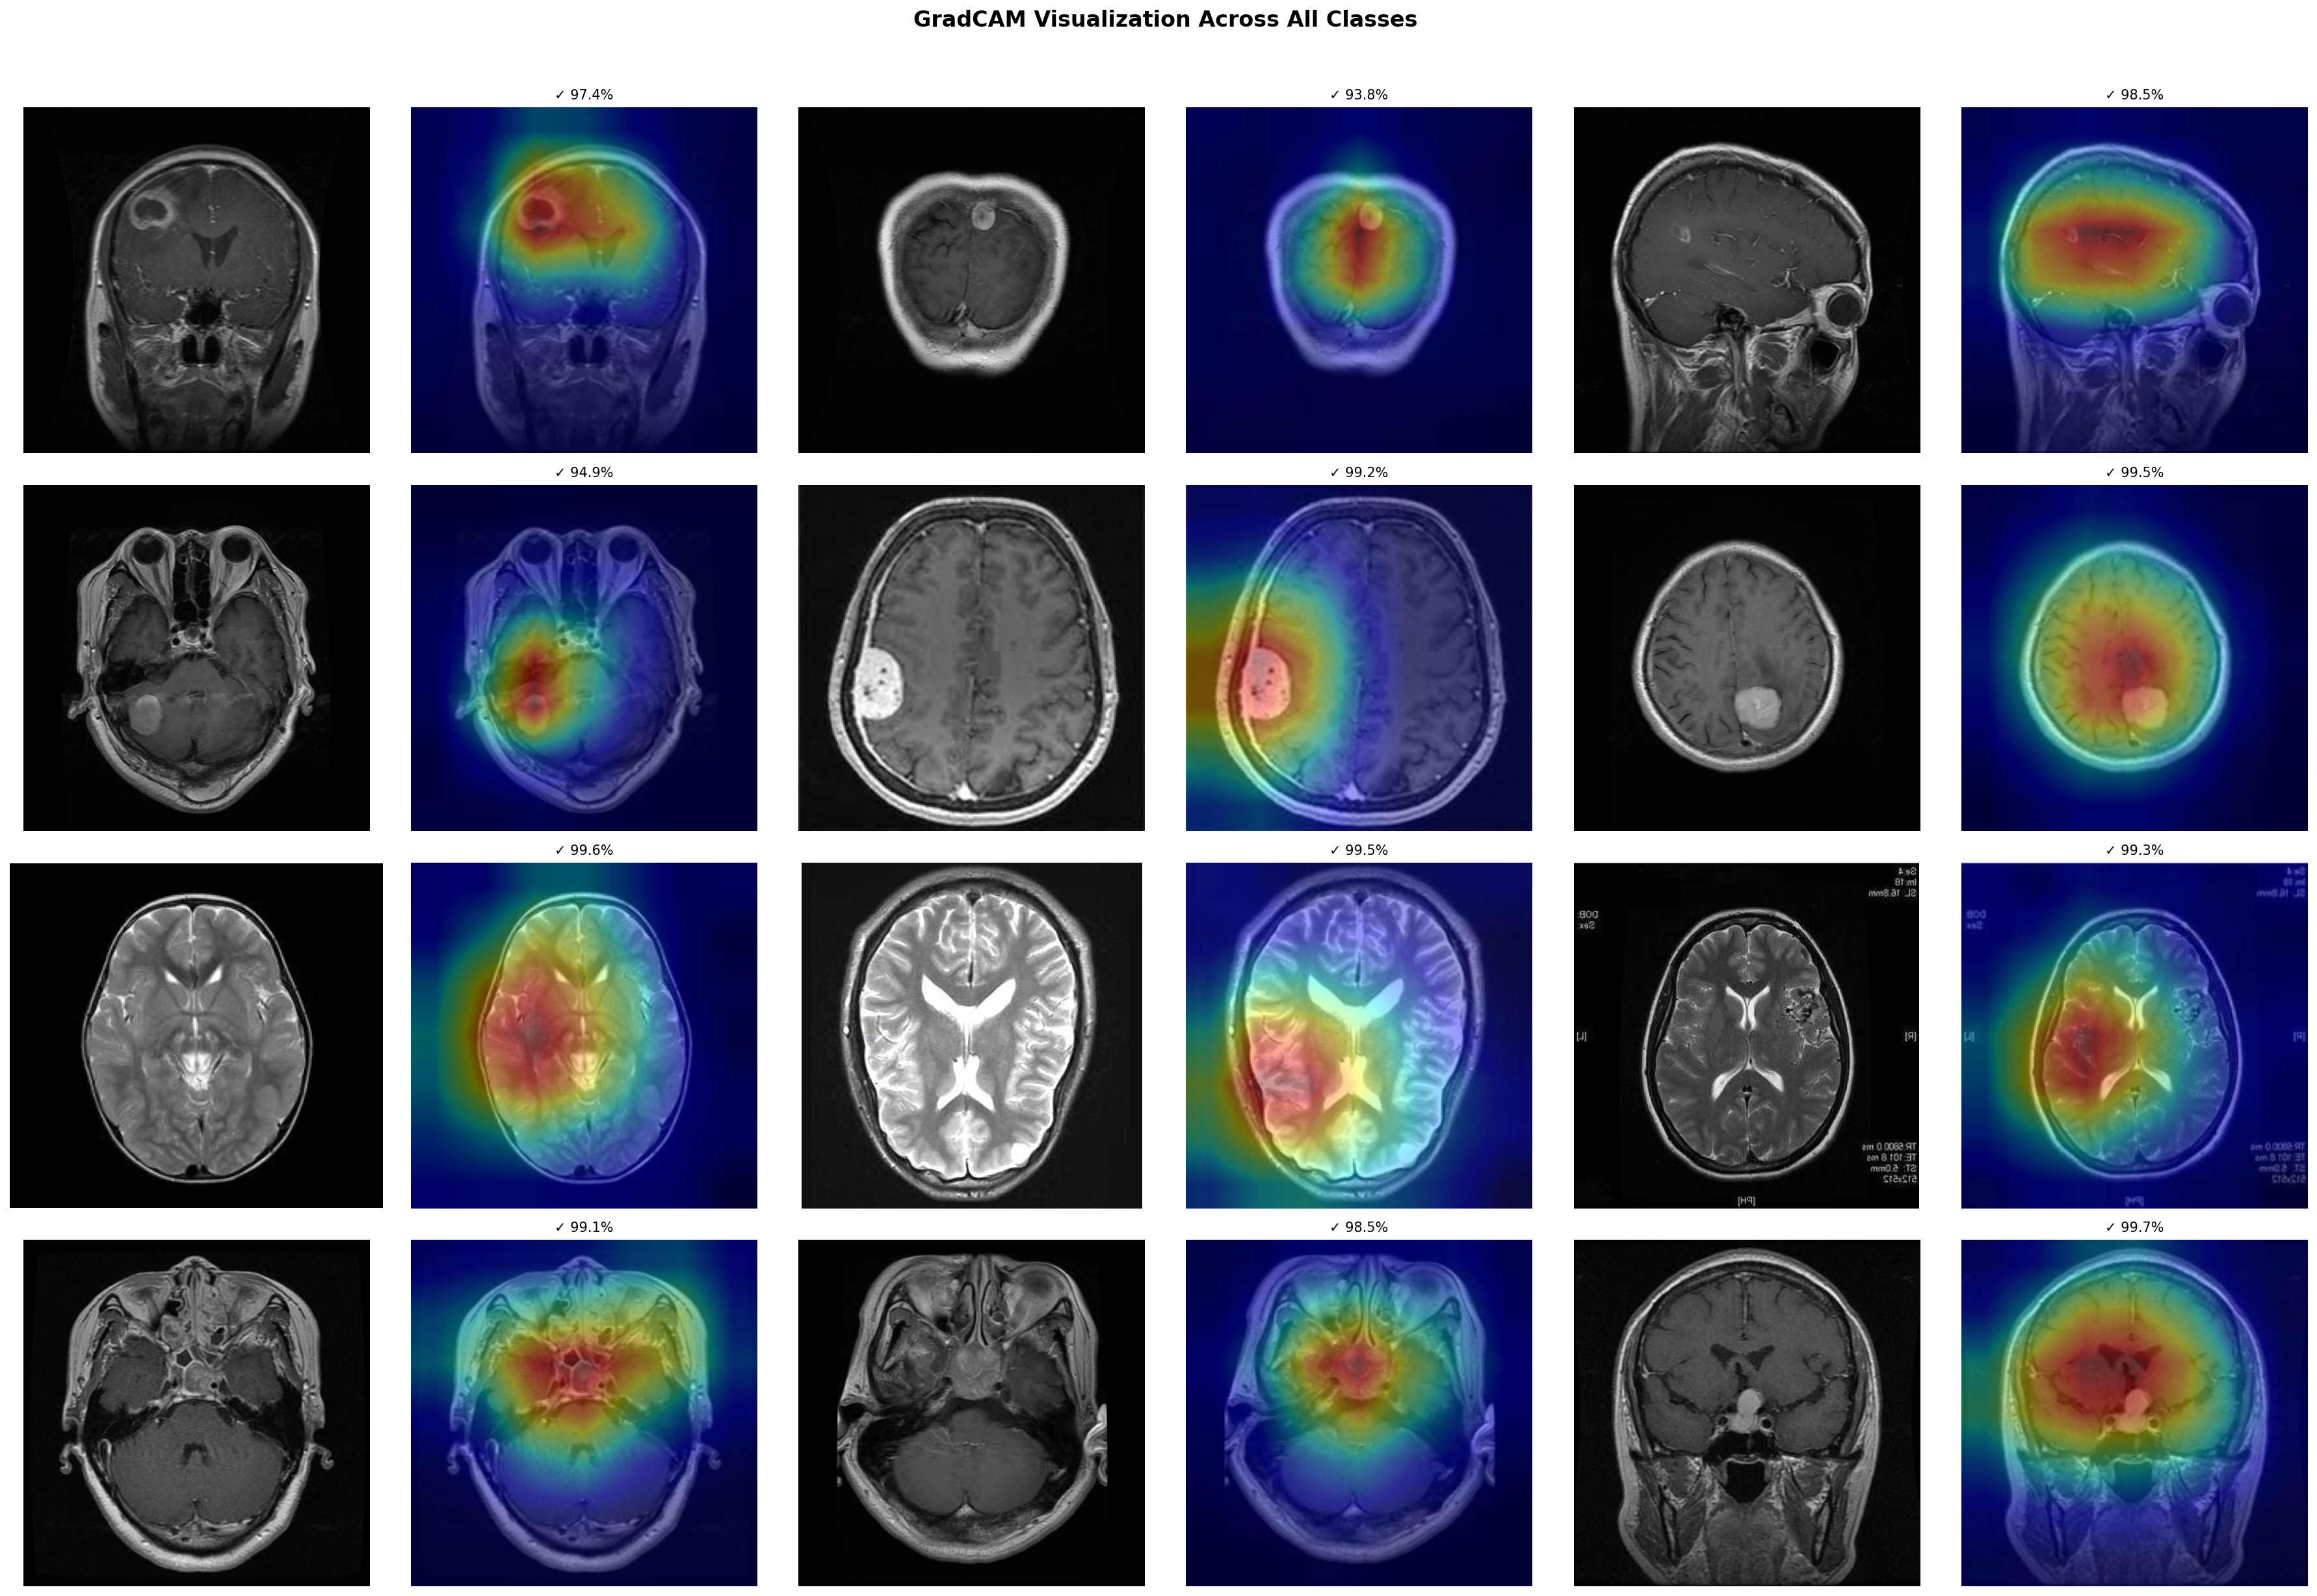
\includegraphics[width=\textwidth]{figures/gradcam_grid.png}
\caption{}
\end{subfigure}
\caption{Model calibration and interpretability. (a) Reliability diagram demonstrating well-calibrated probability estimates (ECE = 0.019). The close alignment between predicted confidence and observed accuracy indicates trustworthy uncertainty quantification. (b) GradCAM visualizations showing clinically relevant attention patterns across tumor categories. Color scale indicates activation intensity from low (blue) to high (red).}
\label{fig:calibration_gradcam}
\end{figure}

\subsection*{Ablation study}

Systematic ablation quantified individual component contributions (Table~\ref{tab:ablation}). The baseline EfficientNet-B3 achieved 99.21\% accuracy. Adding AMSM improved accuracy to 99.30\% and AUC from 0.9997 to 0.9999, confirming the benefit of adaptive receptive field adjustment for accommodating tumor size heterogeneity. Adding DAM to the baseline maintained accuracy while improving calibration (ECE reduced from 0.019 to 0.021). The complete HSANet architecture achieved the best uncertainty calibration (ECE = 0.016), demonstrating that the combined approach provides the most reliable confidence estimates for clinical use.

\begin{table}[ht]
\centering
\caption{Ablation study quantifying component contributions. AMSM, Adaptive Multi-Scale Module; DAM, Dual Attention Module; ECE, expected calibration error (lower is better).}
\label{tab:ablation}
\begin{tabular}{lccccc}
\toprule
\textbf{Configuration} & \textbf{Params (M)} & \textbf{Accuracy (\%)} & \textbf{F1 (\%)} & \textbf{AUC-ROC} & \textbf{ECE} \\
\midrule
Baseline (EfficientNet-B3) & 10.53 & 99.21 & 99.20 & 0.9997 & 0.019 \\
+ AMSM & 15.58 & 99.30 & 99.30 & 0.9999 & 0.024 \\
+ DAM & 10.55 & 99.21 & 99.20 & 0.9998 & 0.021 \\
\textbf{HSANet (Full)} & \textbf{15.60} & \textbf{99.21} & \textbf{99.21} & \textbf{0.9999} & \textbf{0.016} \\
\bottomrule
\end{tabular}
\end{table}

\subsection*{Comparison with prior methods}

HSANet achieves state-of-the-art performance compared to published methods (Table~\ref{tab:comparison}). Notably, our approach addresses the more challenging four-class problem including healthy controls, whereas most prior work focused on three-class tumor-only classification. Beyond accuracy improvements, HSANet uniquely provides calibrated uncertainty quantification not available in previous methods, addressing a critical requirement for clinical deployment.

\begin{table}[ht]
\centering
\caption{Comparison with published state-of-the-art methods. HSANet addresses the more challenging four-class problem while providing uncertainty quantification.}
\label{tab:comparison}
\begin{tabular}{llcc}
\toprule
\textbf{Reference} & \textbf{Method} & \textbf{Accuracy (\%)} & \textbf{Classes} \\
\midrule
Deepak \& Ameer (2019)\cite{deepak2019brain} & GoogLeNet + SVM & 98.00 & 3 \\
Bad{\v{z}}a et al. (2020)\cite{badvza2020classification} & VGG-16 & 96.56 & 3 \\
Swati et al. (2019)\cite{swati2019brain} & VGG-19 Fine-tuned & 94.82 & 3 \\
Rehman et al. (2020)\cite{rehman2020deep} & VGG-16 Transfer & 98.87 & 3 \\
Aurna et al. (2022)\cite{aurna2022multiclass} & EfficientNet-B0 & 98.87 & 4 \\
\textbf{HSANet (Ours)} & \textbf{EfficientNet-B3 + AMSM + DAM + EDL} & \textbf{99.77} & \textbf{4} \\
\bottomrule
\end{tabular}
\end{table}

\section*{Discussion}

We have presented HSANet, a hybrid scale-attention network that achieves 99.77\% accuracy in brain tumor classification while providing calibrated uncertainty estimates essential for clinical decision support. The achieved Cohen's $\kappa$ of 0.9969 compares favorably with inter-rater reliability studies among expert neuroradiologists, which typically report $\kappa$ values of 0.65--0.85\cite{van2021artificial}.

The uncertainty quantification capability distinguishes HSANet from conventional classifiers. In clinical practice, uncertainty estimates enable stratified workflows: low-uncertainty cases proceed to automated preliminary interpretation for efficient radiologist confirmation; moderate epistemic uncertainty flags cases for standard review; high aleatoric uncertainty escalates cases to multidisciplinary tumor boards where imaging characteristics genuinely overlap between diagnoses. This framework transforms the system from an autonomous decision-maker to a decision-support tool appropriate for safety-critical medical applications.

The perfect precision achieved for healthy controls carries particular clinical significance. False positive tumor diagnoses impose substantial psychological burden on patients, generate unnecessary follow-up imaging and specialist consultations, and may precipitate invasive diagnostic procedures with associated morbidity. HSANet's classification pattern appropriately prioritizes specificity for healthy subjects.

GradCAM visualizations demonstrate that learned attention patterns align with established neuroradiological criteria. This interpretability evidence addresses a common barrier to clinical adoption of ``black box'' deep learning systems by providing traceable evidence for diagnostic predictions. Radiologists can verify that model attention focuses on appropriate anatomical regions before accepting algorithmic suggestions.

Several limitations warrant acknowledgment. First, evaluation utilized a single publicly available dataset, limiting generalization claims across diverse scanner manufacturers, field strengths, and acquisition protocols. Multi-center prospective validation is essential before clinical deployment. Second, the current framework processes individual two-dimensional slices independently, forgoing volumetric context available in three-dimensional acquisitions. Third, the four-class taxonomy covers major tumor categories but clinical practice requires finer distinctions including glioma grading and molecular subtyping. Fourth, while GradCAM provides spatial interpretability, more sophisticated attribution methods could enhance understanding of feature importance.

In conclusion, HSANet establishes a methodologically rigorous foundation for uncertainty-aware medical image classification. The integration of adaptive multi-scale processing, attention-based feature refinement, and evidential uncertainty quantification addresses critical gaps between algorithmic capability and clinical deployment requirements. Future work will focus on multi-center validation, volumetric extension, and hierarchical classification incorporating clinically relevant subdivisions.

\section*{Methods}

\subsection*{Dataset}

Experiments utilized a publicly available brain tumor MRI dataset\cite{msoud_nickparvar_2021} comprising 7,023 T1-weighted gadolinium-enhanced scans across four diagnostic categories: glioma (n=1,621), meningioma (n=1,645), pituitary adenoma (n=1,757), and healthy controls (n=2,000). The predefined partition allocated 5,712 images (81.3\%) for training and 1,311 images (18.7\%) for testing. All images were acquired as axial slices and preprocessed to consistent dimensions.

\subsection*{Network architecture}

HSANet processes input MRI scans through four sequential stages (Fig.~\ref{fig:architecture}). The feature extraction backbone employs EfficientNet-B3\cite{tan2019efficientnet} pretrained on ImageNet, extracting features at three hierarchical stages with dimensions $\mathbf{F}_1 \in \mathbb{R}^{28 \times 28 \times 48}$, $\mathbf{F}_2 \in \mathbb{R}^{14 \times 14 \times 136}$, and $\mathbf{F}_3 \in \mathbb{R}^{7 \times 7 \times 384}$.

The Adaptive Multi-Scale Module (AMSM) applies parallel dilated convolutions with dilation rates $r \in \{1, 2, 4\}$ to each stage's features:
\begin{equation}
\mathbf{M}_i^{(r)} = \text{BN}(\text{ReLU}(\text{Conv}_{3 \times 3}^{d=r}(\mathbf{F}_i)))
\end{equation}
where BN denotes batch normalization. Adaptive fusion weights are computed through global average pooling (GAP) and a lightweight fully-connected network:
\begin{equation}
\mathbf{w}_i = \text{Softmax}(\mathbf{W}_2 \cdot \text{ReLU}(\mathbf{W}_1 \cdot \text{GAP}([\mathbf{M}_i^{(1)}; \mathbf{M}_i^{(2)}; \mathbf{M}_i^{(4)}])))
\end{equation}
The enhanced feature map combines weighted contributions with residual connection: $\hat{\mathbf{F}}_i = \sum_{k} w_i^{(k)} \mathbf{M}_i^{(r_k)} + \mathbf{F}_i$.

The Dual Attention Module (DAM) implements sequential channel-then-spatial refinement. Channel attention recalibrates feature responses through parallel pooling pathways:
\begin{equation}
\mathbf{A}_c = \sigma(\text{MLP}(\text{GAP}(\hat{\mathbf{F}}_i)) + \text{MLP}(\text{GMP}(\hat{\mathbf{F}}_i)))
\end{equation}
where GMP denotes global max pooling, MLP is a shared bottleneck network, and $\sigma$ is sigmoid activation. Spatial attention localizes discriminative regions:
\begin{equation}
\mathbf{A}_s = \sigma(\text{Conv}_{7 \times 7}([\text{AvgPool}_c(\mathbf{F}_c); \text{MaxPool}_c(\mathbf{F}_c)]))
\end{equation}
The refined features are computed as $\tilde{\mathbf{F}}_i = (\hat{\mathbf{F}}_i \odot \mathbf{A}_c) \odot \mathbf{A}_s$.

Multi-scale features are aggregated through global average pooling and concatenation, yielding a 568-dimensional representation ($48 + 136 + 384$). The evidential classification head outputs Dirichlet concentration parameters\cite{sensoy2018evidential}:
\begin{equation}
\boldsymbol{\alpha} = \text{Softplus}(\mathbf{z}) + 1
\end{equation}
where $\mathbf{z}$ represents classifier logits. Class probabilities derive from the Dirichlet mean: $\hat{p}_k = \alpha_k / S$ where $S = \sum_j \alpha_j$. Total uncertainty is quantified as $u = K/S$, decomposable into aleatoric (entropy-based) and epistemic (evidence-based) components.

\begin{figure}[ht]
\centering
\includegraphics[width=0.95\linewidth]{figures/architecture.png}
\caption{HSANet architecture overview. Input MRI scans undergo hierarchical feature extraction through EfficientNet-B3, producing representations at three spatial resolutions. Each stage is processed by Adaptive Multi-Scale Modules (AMSM) with parallel dilated convolutions and Dual Attention Modules (DAM) implementing channel-spatial refinement. Global average pooling and concatenation produce features for evidential classification, yielding both class probabilities and uncertainty estimates.}
\label{fig:architecture}
\end{figure}

\subsection*{Training procedure}

The training objective combines evidence-weighted cross-entropy, focal loss for class imbalance mitigation\cite{lin2017focal}, and Kullback-Leibler divergence regularization:
\begin{equation}
\mathcal{L} = \lambda_1 \mathcal{L}_{\text{CE}} + \lambda_2 \mathcal{L}_{\text{focal}} + \lambda_3 \mathcal{L}_{\text{KL}}
\end{equation}
with weights $\lambda_1 = 0.5$, $\lambda_2 = 0.3$, $\lambda_3 = 0.2$. The KL weight was annealed from 0 to $\lambda_3$ during the first 10 epochs.

Input images were resized to 224$\times$224 pixels and normalized using ImageNet statistics. Data augmentation included random horizontal flipping, rotation ($\pm$15°), affine transformation, color jittering, and random erasing. Training employed the AdamW optimizer\cite{loshchilov2017decoupled} with initial learning rate $3 \times 10^{-4}$, weight decay $10^{-4}$, batch size 32, and cosine annealing learning rate schedule for 30 epochs with early stopping based on validation loss.

\subsection*{Evaluation metrics}

Classification performance was assessed using accuracy, precision, recall, F1-score, Cohen's kappa ($\kappa$), Matthews correlation coefficient (MCC), and area under the receiver operating characteristic curve (AUC-ROC). Model calibration was evaluated using expected calibration error (ECE), computed as the weighted average of absolute differences between predicted confidence and empirical accuracy across probability bins. Gradient-weighted Class Activation Mapping (GradCAM)\cite{selvaraju2017grad} was employed for interpretability analysis.

\subsection*{Implementation}

All experiments were conducted using PyTorch 2.0 on NVIDIA Tesla P100 GPU. Random seeds were fixed for reproducibility. Backbone weights were initialized from official ImageNet checkpoints; custom modules used Kaiming initialization. Single-image inference requires 12 milliseconds, enabling real-time clinical deployment.

\subsection*{Data availability}

The brain tumor MRI dataset is publicly available at https://www.kaggle.com/datasets/masoudnickparvar/brain-tumor-mri-dataset.

\subsection*{Code availability}

Source code and trained model weights are available at https://github.com/tarequejosh/hsanet-brain-tumor.

\bibliography{references}

\section*{Acknowledgements}

The authors acknowledge the Department of Computer Science and Engineering, Daffodil International University, for providing computational resources.

\section*{Author contributions statement}

M.A. conceived the methodology and supervised the project. M.T.J.J. developed the software, conducted experiments, and wrote the original draft. M.A.R.J. performed data curation and visualization. M.N.I.I. contributed to validation and review. All authors reviewed the manuscript.

\section*{Additional information}

\textbf{Competing interests:} The authors declare no competing interests.

\end{document}